\documentclass[11pt,a4paper]{article}

% ============================================================
% AURORA-SR
% RGB Spectral Reconstruction, Drought Inference, and
% Resource-Aware Autonomous Earth Observation
% ============================================================

\usepackage[margin=0.8in]{geometry}
\usepackage{amsmath,amssymb,amsfonts,mathtools,bm}
\usepackage{booktabs}
\usepackage{multirow}
\usepackage{array}
\usepackage{tabularx}
\usepackage{graphicx}
\usepackage{float}
\usepackage{siunitx}
\usepackage{xcolor}
\usepackage{hyperref}
\usepackage{url}
\usepackage{enumitem}
\usepackage{algorithm}
\usepackage{algpseudocode}
\usepackage{microtype}
\usepackage{caption}
\usepackage{subcaption}
\usepackage[section]{placeins}
\usepackage{threeparttable}
\usepackage{listings}
\usepackage{tikz}
\graphicspath{{figures/}}
\DeclareGraphicsExtensions{.pdf,.png,.jpg,.jpeg}
\setcounter{topnumber}{3}
\setcounter{totalnumber}{5}
\renewcommand{\topfraction}{0.9}
\renewcommand{\textfraction}{0.07}
\renewcommand{\floatpagefraction}{0.8}
\usetikzlibrary{
    arrows.meta,
    positioning,
    shapes.geometric,
    fit,
    calc
}

\hypersetup{
    colorlinks=true,
    linkcolor=blue!60!black,
    citecolor=blue!60!black,
    urlcolor=blue!60!black
}

\sisetup{
    detect-all=true,
    round-mode=places,
    round-precision=4
}

% ============================================================
% Commands
% ============================================================

\newcommand{\R}{\mathbb{R}}
\newcommand{\E}{\mathbb{E}}
\newcommand{\Prob}{\mathbb{P}}
\newcommand{\vect}[1]{\bm{#1}}
\newcommand{\mat}[1]{\mathbf{#1}}

\newcommand{\AURORA}{\textsc{AURORA}}
\newcommand{\AURORASR}{\textsc{AURORA-SR}}
\newcommand{\DIU}{\mathrm{DIU}}
\newcommand{\SOC}{\mathrm{SOC}}
\newcommand{\RMSE}{\mathrm{RMSE}}
\newcommand{\MAE}{\mathrm{MAE}}
\newcommand{\NIR}{\mathrm{NIR}}
\newcommand{\SWIR}{\mathrm{SWIR}}
\newcommand{\SWIRone}{\mathrm{SWIR1}}
\newcommand{\SWIRtwo}{\mathrm{SWIR2}}

\newcommand{\argmax}{\operatorname*{arg\,max}}
\newcommand{\argmin}{\operatorname*{arg\,min}}

% ============================================================
% Title
% ============================================================

\title{
\textbf{
AURORA-SR: Connecting RGB Spectral Reconstruction and
Physics-Guided Drought Inference with Autonomous
Earth-Observation Planning
}
}

\author{
Dhruv Ranjan\\
DPS Bangalore South, Bengaluru, India\\
\href{https://orcid.org/0009-0009-5883-4300}{ORCID: 0009-0009-5883-4300}
}

\date{September 2026}

% ============================================================
% Document
% ============================================================

\begin{document}

\maketitle

% ============================================================
% Abstract
% ============================================================

\begin{abstract}

This paper describes AURORA-SR, a research framework that connects
RGB-to-six-band spectral reconstruction and physics-guided temporal
drought inference to resource-aware Earth-observation planning for a
small spacecraft. The perception pipeline reconstructs
$[B,G,R,\NIR,\SWIRone,\SWIRtwo]$ imagery and derives spectral features
including NDVI, NDMI, NDWI, SAVI, EVI, and MSI. A spatial--temporal
classifier combines these features with learned sequence
representations. At the planning level, a Bayesian belief model
expresses observation value as expected information gain, while a
dynamic information-utility (DIU) scheduler considers cloud forecasts,
energy, storage, and future access opportunities.

The paper brings together two existing but not yet end-to-end-coupled
components. In the reproducible FINAL\_PROJECT\_NASA production run, the
2,552-sequence cached dataset produced end-to-end spectral validation MAE
$=0.00990$ and RMSE $=0.02523$. The associated drought classifier
reported accuracy $=0.9373$, ROC-AUC $=0.9526$, and F1 $=0.9339$ at a
validation-selected threshold of $0.61$. These are internal,
class-stratified random-split results: the cache labels are mostly
proxy-derived, and the split is not geographically disjoint. Separately,
the executed region-held-out completion run used four unseen regions and
reported ROC-AUC $=0.9412$ and F1 $=0.6000$ on 56 sequences; a
physics-only baseline reached ROC-AUC $=0.9529$ and F1 $=0.7500$ on the
same partition. These holdout results are more conservative and are
reported as a bounded experiment rather than a global estimate.
Separately,
in a synthetic environmental-field simulator, DIU achieved final field
RMSE $=0.01872$ (95\% bootstrap interval $[0.01769,0.01979]$) across
24 matched runs in the nominal scenario, with cumulative information
gain measured in nats.

The two result sets do not measure a single integrated flight system. The
repository now contains an executed software bridge that ranks forecast
regions by information gain per resource cost and exposes replanning
through the local API, but the drought model's confidence output has not
been calibrated as an observation variance and the bridge does not create
new satellite measurements. We therefore do not claim demonstrated
flight or end-to-end physical performance.

\end{abstract}

\noindent
\textbf{Keywords:}
Earth observation,
autonomous spacecraft,
spectral reconstruction,
RGB-to-multispectral,
drought monitoring,
uncertainty-aware planning,
information gain,
spacecraft scheduling,
CubeSat,
synthetic mission simulation.

% ============================================================
% 1. Introduction
% ============================================================

\section{Introduction}

Earth-observation missions are increasingly constrained not by the
ability to acquire an individual image, but by the interaction between
scientific objectives and spacecraft resources. A target may be
geometrically visible but obscured by cloud. An image may have high
scientific value but consume sufficient energy to threaten a future
observation opportunity. A spacecraft may successfully acquire an image
yet be unable to downlink it before subsequent observations fill the
onboard storage. These effects imply that Earth-observation scheduling
is naturally a coupled decision problem rather than a static ranking
problem.

A second challenge concerns the sensing modality itself. Conventional
RGB imagery provides only three broad spectral channels, whereas
vegetation health, canopy water content, and surface moisture are often
more strongly expressed through spectral combinations involving the
near-infrared and shortwave-infrared regions. Direct multispectral
sensors such as Sentinel-2 can provide these channels
\cite{drusch2012}, but a learned spectral
reconstruction approach offers a possible method for extracting
additional environmental information from RGB observations.

The two problems are usually treated independently. A spectral
reconstruction network is trained to minimize image-level spectral
error, while a spacecraft scheduler is designed to maximize target
priority or observation count. Such a separation ignores a critical
fact:

The value of an observation depends on both what it can measure
and what the spacecraft can afford to acquire.

This motivates \AURORASR{}, a framework for coupling the learned
environmental sensing pipeline to an autonomous spacecraft decision
loop. The perception and planning components are implemented and
evaluated separately in the current project; the end-to-end coupling
described below is a proposed interface.

The proposed information flow is

\begin{equation}
\boxed{
\begin{aligned}
RGB
&\rightarrow \hat{\mathbf S}
\rightarrow \hat{\boldsymbol{\Phi}}
\rightarrow (\hat{x},\Sigma_x)\\
&\rightarrow R_{\mathrm{obs}}
\rightarrow \Delta I
\rightarrow U(a)
\rightarrow a^\star
\rightarrow RGB .
\end{aligned}
}
\end{equation}

Here,
$\hat{\mathbf S}$ is the reconstructed spectrum,
$\hat{\boldsymbol{\Phi}}$ contains derived physical spectral indices,
$\hat{x}$ is the environmental estimate,
$\Sigma_x$ represents predictive uncertainty,
$R_{\mathrm{obs}}$ is the observation covariance,
$\Delta I$ is expected information gain,
$U(a)$ is mission utility, and $a^\star$ is the selected spacecraft
action.

The contributions and status of this work are:

\begin{enumerate}[leftmargin=*]

\item A unified, implementation-oriented architecture connecting RGB
spectral reconstruction and physics-guided drought inference to
autonomous Earth-observation mission planning.

\item A mathematically explicit proposed uncertainty interface in
which calibrated perception uncertainty would propagate into the
spacecraft observation covariance.

\item An entropy-based information objective for selecting
observations according to expected reduction in environmental
uncertainty.

\item A resource-aware planning formulation incorporating energy,
storage, thermal state, cloud probability, execution risk, and future
observation opportunities.

\item Separate empirical results for drought inference and the
synthetic AURORA mission simulator, with the distinction between these
experiments retained throughout.

\item A reproducible matched-seed evaluation protocol for the
spacecraft component and an explicit end-to-end protocol for future
integration.

\end{enumerate}

% ============================================================
% 2. Related Work
% ============================================================

\section{Related Work}

\subsection{Spectral Reconstruction}

Spectral reconstruction attempts to infer unavailable spectral
information from measurements containing fewer channels than the
desired output representation. Deep convolutional architectures,
residual networks, attention mechanisms, and transformer-based models
have all been investigated for hyperspectral and multispectral
reconstruction. Residual connections and channel recalibration provide
the architectural foundations used here
\cite{he2016deep,hu2018squeeze}.

The present work differs from a conventional reconstruction benchmark
in that the reconstructed spectrum is not the final product. Instead,
the reconstruction is used to estimate a physical environmental state,
and the uncertainty in that estimate subsequently influences a
spacecraft decision. The uncertainty-aware planner connection is
formulated here but has not yet been evaluated end to end.

\subsection{Physics-Guided Remote Sensing}

Explicit spectral indices such as NDVI and NDMI provide interpretable
relationships between spectral measurements and vegetation or
moisture conditions. Incorporating these quantities into learned models
provides an intermediate representation connecting data-driven
features with known physical relationships \cite{rouse1974,gao1996,
mcfeeters1996,huete1988,huete2002}.

The present architecture uses these indices as auxiliary information
rather than treating them as replacements for learned features.

\subsection{Autonomous Earth Observation}

Autonomous spacecraft planning has been studied through automated
science selection and observation scheduling
\cite{chien2005autonomous}. Bayesian filtering and information theory
provide standard tools for representing state uncertainty and
quantifying information gain \cite{kalman1960,shannon1948}.

The distinguishing feature of \AURORASR{} is the explicit coupling of
the observation model to the learned environmental inference process.
An observation is valuable because it reduces uncertainty in an
environmental state, not simply because a target has been assigned a
large static priority. This coupling is the proposed next integration
step, rather than a result of the current simulator experiments.

% ============================================================
% 3. Problem Formulation
% ============================================================

\section{Problem Formulation}

Let the environmental state at time $t$ be

\begin{equation}
\vect{x}_t
=
\begin{bmatrix}
x_{1,t} &
x_{2,t} &
\cdots &
x_{N,t}
\end{bmatrix}^{\mathsf T},
\end{equation}

where $x_{i,t}\in[0,1]$ represents the drought state or drought
probability associated with target $i$.

The spacecraft state is

\begin{equation}
\vect{s}_t
=
\begin{bmatrix}
\vect{r}_t &
\vect{v}_t &
B_t &
S_t &
T_t &
q_t
\end{bmatrix}^{\mathsf T},
\end{equation}

where $\vect r_t$ and $\vect v_t$ are position and velocity,
$B_t$ is battery energy, $S_t$ is onboard data storage, $T_t$ is
thermal state, and $q_t$ represents attitude or pointing state.

The complete state evolves according to

\begin{align}
\vect{x}_{t+1}
&=
f_x(\vect{x}_t,\vect{w}_t),\\
\vect{s}_{t+1}
&=
f_s(\vect{s}_t,a_t,\vect{v}_t),
\end{align}

where $a_t$ is a spacecraft action.

An observation produces

\begin{equation}
z_t
=
h(\vect{x}_t,a_t)
+
\epsilon_t.
\end{equation}

The central optimization problem is

\begin{equation}
\boxed{
\pi^\star
=
\argmax_{\pi}
\E_\pi
\left[
\sum_{t=0}^{H}
U(\vect{x}_t,\vect{s}_t,a_t)
\right]
}
\end{equation}

subject to

\begin{align}
B_t &\geq B_{\min},\\
S_t &\leq S_{\max},\\
T_{\min} &\leq T_t \leq T_{\max},\\
a_t &\in\mathcal{A}_t,
\end{align}

where $\mathcal A_t$ contains only geometrically and operationally
feasible actions.

% ============================================================
% 4. Overall Architecture
% ============================================================

\section{AURORA-SR Architecture}

The complete system consists of five layers:

\begin{enumerate}[leftmargin=*]

\item \textbf{Spectral reconstruction:}
RGB imagery is mapped to a six-band spectral representation.

\item \textbf{Physics-guided environmental inference:}
reconstructed spectral bands are transformed into physically meaningful
indices and temporal features.

\item \textbf{Probabilistic state estimation:}
drought predictions and their uncertainty are converted into a
Bayesian environmental belief state.

\item \textbf{Spacecraft simulation:}
orbital geometry and spacecraft resources determine which observations
are physically feasible.

\item \textbf{Autonomous planning:}
the DIU planner chooses the observation expected to provide the largest
scientific information return while respecting spacecraft constraints.

\end{enumerate}

In the current repository, the perception model and the AURORA mission
simulator are separately executable components. The dashed interface
in Fig.~\ref{fig:architecture} is a proposed integration boundary: a
calibrated variance estimate must be produced and validated before the
perception output can be used as a probabilistic planner measurement.

\begin{figure}[!htbp]
\centering

\resizebox{\linewidth}{!}{%
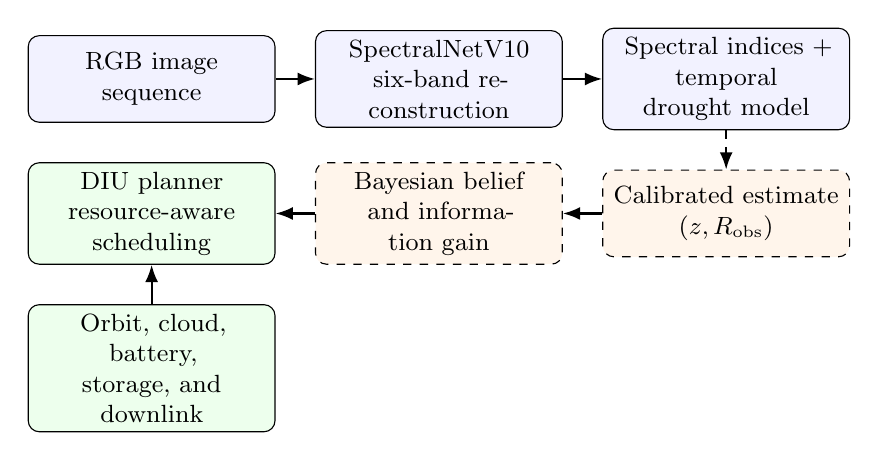
\begin{tikzpicture}[
node distance=5mm,
box/.style={draw,rounded corners,align=center,text width=2.9cm,
minimum height=11mm,font=\small,fill=blue!5},
proposed/.style={draw,dashed,rounded corners,align=center,
text width=2.9cm,minimum height=11mm,font=\small,fill=orange!8},
simulator/.style={draw,rounded corners,align=center,
text width=2.9cm,minimum height=11mm,font=\small,fill=green!7},
arrow/.style={-{Latex[length=2.2mm]},thick}
]
\node[box] (rgb) {RGB image sequence};
\node[box,right=of rgb] (spectral) {SpectralNetV10\\
six-band reconstruction};
\node[box,right=of spectral] (drought) {Spectral indices +\\
temporal drought model};
\node[proposed,below=of drought] (measurement) {Calibrated estimate\\
$(z,R_{\mathrm{obs}})$};
\node[proposed,left=of measurement] (belief) {Bayesian belief\\
and information gain};
\node[simulator,left=of belief] (planner) {DIU planner\\
resource-aware scheduling};
\node[simulator,below=of planner] (mission) {Orbit, cloud, battery,\\
storage, and downlink};
\draw[arrow] (rgb) -- (spectral);
\draw[arrow] (spectral) -- (drought);
\draw[arrow,dashed] (drought) -- (measurement);
\draw[arrow] (measurement) -- (belief);
\draw[arrow] (belief) -- (planner);
\draw[arrow] (mission) -- (planner);

\end{tikzpicture}
}

\caption{
Implemented components (blue perception; green mission simulator) and
the proposed probabilistic interface (orange, dashed). The current
classifier confidence output is not a calibrated observation variance;
the dashed connection must be completed and tested before claiming
end-to-end AURORA-SR performance. A selected observation would initiate
the next acquisition cycle.
}

\label{fig:architecture}
\end{figure}

% ============================================================
% 5. Spectral Reconstruction
% ============================================================

\section{RGB Spectral Reconstruction}

\subsection{Input and Target Representation}

Let the RGB observation at time $t$ be

\begin{equation}
\vect{I}^{RGB}_t
\in
[0,1]^{3\times H\times W}.
\end{equation}

The desired spectral representation is

\begin{equation}
\vect{S}_t
=
[
B_t,
G_t,
R_t,
NIR_t,
SWIR1_t,
SWIR2_t
]^{\mathsf T}.
\end{equation}

The spectral reconstruction network learns

\begin{equation}
\hat{\vect{S}}_t
=
f_\theta
\left(
\vect{I}^{RGB}_t
\right).
\end{equation}

The implementation applies the image model independently to each
frame in a sequence:

\begin{equation}
\hat{\vect{S}}_{1:T}
=
\{f_\theta(\vect{I}^{RGB}_t)\}_{t=1}^{T}.
\end{equation}

The three visible output channels are formed by reordering the RGB
input to $[B,G,R]$ and adding a bounded learned correction; the three
inferred channels are passed through a sigmoid. Thus, the visible bands
are not an unconstrained copy of the input, and the NIR/SWIR channels
remain model estimates rather than direct measurements.

\subsection{Residual Encoder}

The supplied SpectralNetV10 model uses a residual encoder--decoder
with squeeze-and-excitation channel attention.

For an input feature map $\vect X$,

\begin{equation}
\vect F
=
\mathcal{C}_2
\left[
\phi
\left(
\mathcal{C}_1(\vect X)
\right)
\right],
\end{equation}

where $\mathcal C_1$ and $\mathcal C_2$ are convolutional mappings.

The residual output is

\begin{equation}
\vect Y
=
\phi\left(\mathcal P(\vect X)+\vect F\right),
\end{equation}

where $\mathcal P$ is the identity when channel dimensions match and a
learned $1\times1$ projection otherwise. Here $\vect F$ denotes the
two-convolution branch after squeeze-and-excitation recalibration.
The activation $\phi$ is the block's ReLU; this matches the
implementation's projected shortcut and post-addition activation.

\subsection{Squeeze-and-Excitation}

For $\vect X\in\R^{C\times H\times W}$, channel statistics are

\begin{equation}
z_c
=
\frac{1}{HW}
\sum_{h=1}^{H}
\sum_{w=1}^{W}
X_{c,h,w}.
\end{equation}

The excitation vector is

\begin{equation}
\vect e
=
\sigma
\left[
W_2
\delta
\left(
W_1\vect z
\right)
\right],
\end{equation}

where $\delta$ is the nonlinear activation.

The recalibrated feature map becomes

\begin{equation}
\tilde X_{c,h,w}
=
e_cX_{c,h,w}.
\end{equation}

\subsection{Multiscale Reconstruction}

The training implementation uses band weights
$\vect w=[1,1,1,1.2,1.2,1.2]$ to emphasize the inferred channels. For
pixelwise prediction $\hat{\vect S}$ and target $\vect S$, the primary
loss is

\begin{equation}
\mathcal L_{\mathrm{main}}
=
\operatorname{mean}
\left[
\vect w\odot(\hat{\vect S}-\vect S)^2
\right]
+0.1\,\operatorname{SmoothL1}(\hat{\vect S},\vect S).
\end{equation}

Two auxiliary decoder outputs are interpolated to the target resolution
and supervised against the same spectral target. The implemented
objective is

\begin{equation}
\boxed{
\mathcal L_{SR}
=
\mathcal L_{\mathrm{main}}
+0.30\left[
\operatorname{MSE}(\hat{\vect S}^{(mid)},\vect S)
+
\operatorname{MSE}(\hat{\vect S}^{(low)},\vect S)
\right].
}
\end{equation}

\begin{figure}[!htbp]
\centering
\resizebox{\linewidth}{!}{%
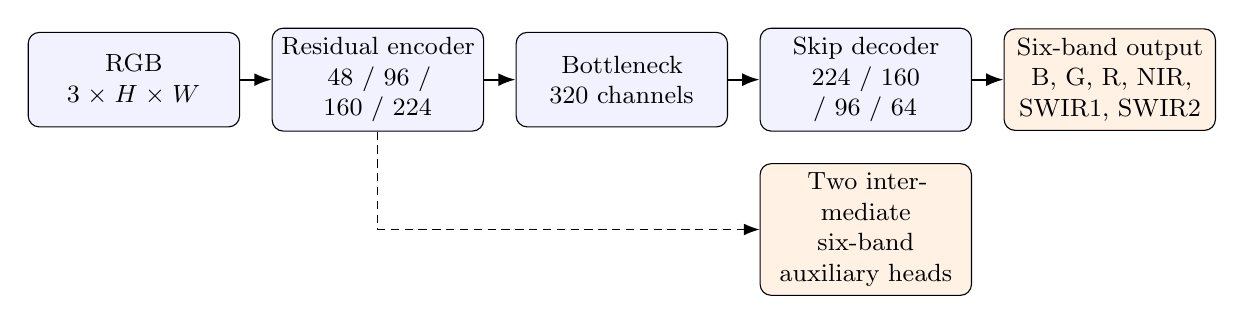
\begin{tikzpicture}[
node distance=4mm,
layer/.style={draw,rounded corners,align=center,text width=2.45cm,
minimum height=12mm,font=\small,fill=blue!5},
head/.style={draw,rounded corners,align=center,text width=2.45cm,
minimum height=12mm,font=\small,fill=orange!10},
arr/.style={-{Latex[length=2.2mm]},thick},
skip/.style={-{Latex[length=2mm]},thin,densely dashed}
]
\node[layer] (input) {RGB\\$3\times H\times W$};
\node[layer,right=of input] (enc) {Residual encoder\\
48 / 96 / 160 / 224};
\node[layer,right=of enc] (bottleneck) {Bottleneck\\320 channels};
\node[layer,right=of bottleneck] (dec) {Skip decoder\\
224 / 160 / 96 / 64};
\node[head,right=of dec] (out) {Six-band output\\
B, G, R, NIR, SWIR1, SWIR2};
\node[head,below=of dec] (aux) {Two intermediate\\
six-band auxiliary heads};
\draw[arr] (input) -- (enc);
\draw[arr] (enc) -- (bottleneck);
\draw[arr] (bottleneck) -- (dec);
\draw[arr] (dec) -- (out);
\draw[skip] (enc.south) |- (aux.west);
\end{tikzpicture}
}
\caption{SpectralNetV10 encoder--decoder and auxiliary supervision.
Each residual stage includes squeeze-and-excitation channel
recalibration. The auxiliary outputs are bilinearly upsampled and
trained against the six-band target; they are not additional
observations.}
\label{fig:spectral-network}
\end{figure}

\subsection{Spectral Metrics}

Mean absolute error is

\begin{equation}
\mathrm{MAE}
=
\frac{1}{N}
\sum_{i=1}^{N}
\left|
\hat{s}_i-s_i
\right|.
\end{equation}

Root mean square error is

\begin{equation}
\mathrm{RMSE}
=
\sqrt{
\frac{1}{N}
\sum_{i=1}^{N}
(\hat{s}_i-s_i)^2
}.
\end{equation}

Spectral angle mapper error is

\begin{equation}
\mathrm{SAM}
=
\cos^{-1}
\left(
\frac{
\hat{\vect{s}}^\mathsf T\vect{s}
}{
\|\hat{\vect{s}}\|_2
\|\vect{s}\|_2+\epsilon
}
\right).
\end{equation}

The validation results for these metrics are reported in
Table~\ref{tab:spectral-results}.

% ============================================================
% 6. Physics Guided Drought Model
% ============================================================

\section{Physics-Guided Drought Inference}

\subsection{Implemented Spectral Features}

The normalized difference vegetation index (NDVI)
\cite{rouse1974} is

\begin{equation}
NDVI
=
\frac{
NIR-R
}{
NIR+R+\epsilon
}.
\end{equation}

\subsection{Normalized Difference Moisture Index}

The normalized difference moisture index (NDMI) follows Gao
\cite{gao1996}:

\begin{equation}
NDMI
=
\frac{
NIR-SWIR1
}{
NIR+SWIR1+\epsilon
}.
\end{equation}

\subsection{Normalized Difference Water Index}

The green--NIR normalized difference water index (NDWI)
\cite{mcfeeters1996} is

\begin{equation}
NDWI
=
\frac{
G-NIR
}{
G+NIR+\epsilon
}.
\end{equation}

\subsection{Soil Adjusted Vegetation Index}

The implementation fixes the soil adjustment parameter to $L=0.5$
\cite{huete1988}:

\begin{equation}
SAVI
=
\left(1+0.5\right)
\frac{
NIR-R
}{
NIR+R+0.5+\epsilon
}.
\end{equation}

\subsection{Enhanced Vegetation Index}

The implementation uses the standard coefficients
\cite{huete2002}:

\begin{equation}
EVI
=
2.5
\frac{
NIR-R
}{
NIR+6R-7.5B+1+\epsilon
}.
\end{equation}

\subsection{Moisture Stress Index}

\begin{equation}
MSI
=
\frac{
SWIR1
}{
NIR+\epsilon
}.
\end{equation}

The implementation also derives the normalized burn ratio
$NBR=(NIR-SWIR2)/(NIR+SWIR2+\epsilon)$, the green chlorophyll
indicator $GCI=NIR/(G+\epsilon)-1$, and the linear terms
$NIR-SWIR1$, $G-R$, $NIR-SWIR2$, and $SWIR1-NIR$. Together with the
six input bands, these form an 18-channel feature image for each frame.
All ratios use $\epsilon=10^{-6}$ in the drought feature builder.
These indices are proxies for vegetation, water, and moisture
conditions; their values inherit any error in the reconstructed bands.

% ============================================================
% 7. Physics Prior
% ============================================================

\subsection{Physics-Derived Drought Prior}

Let

\begin{equation}
\vect{\phi}_t
=
\begin{bmatrix}
NDVI_t & NDMI_t & NDWI_t & NBR_t & SAVI_t & EVI_t\\
MSI_t & GCI_t & NIR_t-SWIR1_t & G_t-R_t
& NIR_t-SWIR2_t & SWIR1_t-NIR_t
\end{bmatrix}^{\mathsf T}.
\end{equation}

Spatial means of the derived features are computed at each sequence
step. The prior uses the last-step value, the first-to-last change,
the sequence mean, and the temporal range. For a scalar feature $v$,
the implementation maps a reference ``good'' value $g$ and a
stress-side ``bad'' value $b$ to

\begin{equation}
\operatorname{stress}(v;g,b)
=
\operatorname{clip}\left(
\frac{v-g}{b-g},0,1\right)
\quad (b>g),
\end{equation}
with the numerator and denominator signs reversed when $b<g$. The
physics prior is the following fixed weighted sum of normalized
stress terms:

\begin{equation}
p_{\mathrm{phys}}
=
\operatorname{clip}\left(
\begin{aligned}
0.20s_{\mathrm{veg}}
&+0.17s_{\mathrm{moist}}\\
&+0.07s_{\mathrm{water}}+0.07s_{\mathrm{NBR}}\\
&+0.08s_{\mathrm{SAVI}}+0.08s_{\mathrm{MSI}}
+0.05s_{\mathrm{soil}}\\
&+0.12s_{\Delta\mathrm{NDVI}}
+0.08s_{\Delta\mathrm{NDMI}}
+0.03s_{\Delta\mathrm{NDWI}}\\
&+0.03s_{\Delta\mathrm{NBR}}
+0.02s_{\Delta\mathrm{SAVI}}
\end{aligned},
0,1\right).
\end{equation}

The corresponding reference thresholds and weights are:

\begin{table}[!htbp]
\centering
\caption{Fixed heuristic thresholds used to construct the drought
physics prior. ``Good $\rightarrow$ stress'' lists the input values
mapped to prior values 0 and 1, respectively.}
\label{tab:prior-terms}
\begin{tabular}{lccc}
\toprule
Term & Feature & Good $\rightarrow$ stress & Weight\\
\midrule
Low vegetation & last NDVI & $0.58\rightarrow0.12$ & 0.20\\
Low moisture & last NDMI & $0.20\rightarrow-0.12$ & 0.17\\
Low surface water & last NDWI & $0.10\rightarrow-0.18$ & 0.07\\
Burn/dryness & last NBR & $0.48\rightarrow0.06$ & 0.07\\
Canopy loss & last SAVI & $0.46\rightarrow0.08$ & 0.08\\
Moisture stress & last MSI & $0.55\rightarrow1.35$ & 0.08\\
Dry soil & last $(SWIR1-NIR)$ & $-0.18\rightarrow0.18$ & 0.05\\
Vegetation decline & first--last NDVI & $0.00\rightarrow0.16$ & 0.12\\
Moisture decline & first--last NDMI & $0.00\rightarrow0.12$ & 0.08\\
Water decline & first--last NDWI & $0.00\rightarrow0.10$ & 0.03\\
NBR decline & first--last NBR & $0.00\rightarrow0.12$ & 0.03\\
SAVI decline & first--last SAVI & $0.00\rightarrow0.16$ & 0.02\\
\bottomrule
\end{tabular}
\end{table}

These fixed thresholds are code-level heuristics, not thresholds
estimated from independently observed drought outcomes. The prior is
an auxiliary feature and regularizer; it must not be interpreted as
an independent ground-truth label.

% ============================================================
% 8. Temporal Model
% ============================================================

\section{Temporal Drought Model}

For a sequence of $T$ observations, the implementation computes the
18-channel spectral-feature image $\vect F_t$ at each time step and
summarizes its spatial mean and standard deviation. A convolutional
spatial encoder augments these statistics to form frame embeddings
$\vect e_t$. The recurrent branch is a two-layer bidirectional GRU
\cite{cho2014}; a parallel temporal convolution provides a second
branch.

\begin{equation}
\begin{aligned}
\vect C_{1:T}
&=\operatorname{Conv1D}(\vect e_{1:T}),\\
\vect H_{1:T}
&=\operatorname{BiGRU}_{2\text{-layer}}(\vect e_{1:T}).
\end{aligned}
\end{equation}

Learned attention over the bidirectional GRU outputs produces
$\vect h_{\mathrm{attn}}$; the model also retains the last GRU state and
the pooled and last convolutional features. A separate multilayer
perceptron embeds a 33-element physics vector comprising last-step,
change, sequence-mean and sequence-range summaries plus $p_{\mathrm{phys}}$.
The final classifier is

\begin{equation}
\hat p=\sigma\left(
f_{\mathrm{head}}[
\vect h_{\mathrm{attn}};
\vect h_T;
\operatorname{mean}(\vect C);
\vect C_T;
f_{\mathrm{phys}}(\vect q)]
\right).
\end{equation}

Training uses a class-balanced sampler and a weighted composite
objective. For hard labels $y$, soft targets $y_s$, label confidence
$c_y$, classifier probability $p$, auxiliary confidence prediction
$p_c$, and physics prior $p_{\mathrm{phys}}$, the per-sample loss is

\begin{equation}
\ell
=
(0.35+0.65c_y)
\left[
0.55\ell_{\mathrm{focal}}(p,y)
 + 0.20|p-y_s|
 + 0.15|p_c-c^\star|
 + 0.10|p-p_{\mathrm{phys}}|
\right],
\end{equation}
where $\ell_{\mathrm{focal}}$ uses $\alpha=0.75$, $\gamma=2$
\cite{lin2017}, and
$c^\star=\operatorname{clip}(0.65|2y_s-1|+
0.35|2p_{\mathrm{phys}}-1|,0,1)$. The reported confidence head is
trained to this constructed target. It is not an aleatoric variance,
has not been calibration-tested, and cannot yet be inserted directly
as $R_{\mathrm{obs}}$.

\subsection{Evaluation Rule}

Quantitative performance and the confusion counts are reported in
Table~\ref{tab:drought-validation}. The threshold is selected for
maximum F1 on the internal validation partition.

% ============================================================
% 9. Probabilistic Sensor
% ============================================================

\section{Proposed Probabilistic Environmental Sensor Interface}

The proposed planner interface avoids treating the learned
environmental estimate as a perfect observation. The current drought
pipeline does not produce a calibrated variance, so the following
observation model is a design specification rather than an implemented
or evaluated connection.

For target $i$, the desired perception output is

\begin{equation}
\mathcal O_i
=
\left(
\hat{x}_i,
\Sigma_{SR,i},
q_i,
c_i
\right),
\end{equation}

where $\hat{x}_i$ is estimated drought probability,
$\Sigma_{SR,i}$ is calibrated predictive uncertainty, $q_i$ is
observation quality, and $c_i$ is cloud probability. The current
confidence head is a score trained against a constructed proxy target;
it must not be substituted for $\Sigma_{SR,i}$ without calibration.

If a spectral predictive covariance $\Sigma_{S,i}$ is available, a
first-order propagation through the drought estimator $h$ is

\begin{equation}
\Sigma_{SR,i}
\approx
J_{h,i}\Sigma_{S,i}J_{h,i}^{\mathsf T}
+\Sigma_{\mathrm{res},i},
\end{equation}
where $J_{h,i}$ is the local Jacobian and
$\Sigma_{\mathrm{res},i}$ represents residual model uncertainty. This
approximation requires empirical calibration and testing under
geographic, seasonal, and cloud shifts.

For a scalar environmental state and approximately independent error
sources, the proposed local measurement model is

\begin{equation}
z_i=x_i+v_i,\qquad v_i\sim\mathcal N(0,R_i).
\end{equation}

The proposed effective measurement variance is

\begin{equation}
\boxed{
R_i
=
R_{\mathrm{sensor}}
+ \sigma^2_{SR,i}
+
R_{\mathrm{cloud},i}
+ R_{\mathrm{model},i}.
}
\end{equation}

Additivity is an explicit simplifying assumption. The Gaussian model
approximates a bounded probability-valued quantity; its adequacy must
be tested before planner results can be interpreted.

% ============================================================
% 10. Uncertainty Estimation
% ============================================================

\subsection{Candidate Heteroscedastic Uncertainty Model}

One candidate future estimator adds a variance head
\cite{kendall2017}:

\begin{align}
\hat{x}_i
&=
\sigma(f_\mu(\vect I_i)),\\
\log \hat{\sigma}_{i}^{2}
&=
f_v(\vect I_i).
\end{align}

For a continuous approximation, a Gaussian negative log-likelihood is

\begin{equation}
\mathcal L_{\mathrm{NLL}}
=
\frac{1}{2}
\left[
\frac{
(y-\mu)^2
}{
\sigma^2
}
+
\log\sigma^2
\right].
\end{equation}

Alternatively, ensemble or Monte Carlo dropout uncertainty can be
used.

The final publication experiment should explicitly compare uncertainty
methods rather than selecting one after observing the final results.

% ============================================================
% 11. AURORA Physics
% ============================================================

\section{AURORA Spacecraft Physics Model}

\subsection{State Vector}

The translational spacecraft state is

\begin{equation}
\vect y
=
\begin{bmatrix}
\vect r\\
\vect v
\end{bmatrix}.
\end{equation}

Under a two-body gravitational model,

\begin{equation}
\dot{\vect r}
=
\vect v,
\end{equation}

and

\begin{equation}
\dot{\vect v}
=
-\frac{\mu_E}
{\|\vect r\|^3}
\vect r.
\end{equation}

The fourth-order Runge--Kutta integration is

\begin{align}
k_1
&=
f(y_t),\\
k_2
&=
f
\left(
y_t+\frac{\Delta t}{2}k_1
\right),\\
k_3
&=
f
\left(
y_t+\frac{\Delta t}{2}k_2
\right),\\
k_4
&=
f
\left(
y_t+\Delta t k_3
\right),
\end{align}

with

\begin{equation}
y_{t+\Delta t}
=
y_t+
\frac{\Delta t}{6}
(k_1+2k_2+2k_3+k_4).
\end{equation}

\subsection{Orbital Energy}

Specific orbital energy is

\begin{equation}
\mathcal E
=
\frac{\|\vect v\|^2}{2}
-
\frac{\mu_E}{\|\vect r\|}.
\end{equation}

The normalized energy error is

\begin{equation}
\epsilon_E
=
\frac{
|\mathcal E_t-\mathcal E_0|
}{
|\mathcal E_0|
}.
\end{equation}

\subsection{Angular Momentum}

Specific angular momentum is

\begin{equation}
\vect h
=
\vect r\times\vect v.
\end{equation}

The normalized angular-momentum error is

\begin{equation}
\epsilon_h
=
\frac{
\|\vect h_t-\vect h_0\|
}{
\|\vect h_0\|
}.
\end{equation}

% ============================================================
% 12. Earth Rotation
% ============================================================

\subsection{Earth Rotation and Ground Track}

The ECI-to-ECEF transformation is approximated by

\begin{equation}
\vect r_{ECEF}
=
R_3(\theta_E)
\vect r_{ECI}.
\end{equation}

The Earth rotation angle is

\begin{equation}
\theta_E(t)
=
\theta_{E,0}
+
\omega_E t.
\end{equation}

For a spherical Earth approximation,

\begin{align}
\lambda
&=
\operatorname{atan2}(y,x),\\
\phi
&=
\operatorname{atan2}
\left(
z,
\sqrt{x^2+y^2}
\right).
\end{align}

% ============================================================
% 13. Eclipse
% ============================================================

\subsection{Solar Geometry and Eclipse}

Let

\begin{equation}
\hat{\vect s}
=
\frac{\vect r_{\odot}-\vect r}
{\|\vect r_{\odot}-\vect r\|}
\end{equation}

be the Sun direction from the spacecraft.

The simplified panel incidence factor is

\begin{equation}
\eta_{\mathrm{inc}}
=
\max
\left(
0,
\hat{\vect n}\cdot\hat{\vect s}
\right).
\end{equation}

Solar power is

\begin{equation}
P_{\mathrm{solar}}
=
P_{\mathrm{BOL}}
\eta_{\mathrm{inc}}
\eta_{\mathrm{deg}}
\eta_{\mathrm{eclipse}}.
\end{equation}

% ============================================================
% 14. Battery
% ============================================================

\section{Spacecraft Resource Model}

\subsection{Battery}

Let $B_t$ denote stored battery energy.

\begin{equation}
B_{t+\Delta t}
=
\operatorname{clip}
\left[
B_t
+
\eta_cP_{charge}\Delta t
-
\frac{P_{load}\Delta t}{\eta_d},
0,
B_{\max}
\right].
\end{equation}

The normalized state of charge is

\begin{equation}
SOC_t
=
\frac{B_t}{B_{\max}}.
\end{equation}

A hard safety constraint is

\begin{equation}
SOC_t
\geq
SOC_{\min}.
\end{equation}

% ============================================================
% 15. Thermal
% ============================================================

\subsection{Thermal State}

This lumped model is a proposed resource constraint for a future
mission-specific integration. It is not active in the publication
simulator experiment summarized in Section~\ref{sec:aurora-protocol}.

A lumped thermal model is

\begin{equation}
C_{th}
\frac{dT}{dt}
=
P_{abs}
-
P_{rad}
-
P_{out},
\end{equation}

where radiative loss may be approximated by

\begin{equation}
P_{rad}
=
\epsilon\sigma A
\left(
T^4-T_{env}^4
\right).
\end{equation}

The mission constraint is

\begin{equation}
T_{\min}
\leq
T_t
\leq
T_{\max}.
\end{equation}

% ============================================================
% 16. Storage
% ============================================================

\subsection{Onboard Storage}

The storage state evolves as

\begin{equation}
S_{t+\Delta t}
=
S_t
+
D_{\mathrm{generated}}
-
D_{\mathrm{downlink}}.
\end{equation}

For an observation requiring $D_{obs}$ bits,

\begin{equation}
S_t+D_{obs}
\leq
S_{\max}.
\end{equation}

% ============================================================
% 17. Observation Opportunities
% ============================================================

\subsection{Observation Geometry}

For target $i$, an observation opportunity is

\begin{equation}
o_{i,t}
=
(
t,
\theta_{off},
e_i,
c_i,
E_i,
D_i
).
\end{equation}

Here $\theta_{off}$ is off-nadir angle,
$e_i$ is geometric elevation,
$c_i$ is cloud probability,
$E_i$ is energy cost, and
$D_i$ is data volume.

Only observations satisfying

\begin{equation}
o_{i,t}\in\mathcal A_t
\end{equation}

are passed to the planner.

% ============================================================
% 18. Bayesian Belief
% ============================================================

\section{Bayesian Environmental State Estimation}

Each target maintains

\begin{equation}
x_i
\sim
\mathcal N(\mu_i,P_i).
\end{equation}

\subsection{Prediction}

A random-walk environmental model is

\begin{equation}
x_{i,t+1}
=
x_{i,t}
+
w_{i,t},
\end{equation}

with

\begin{equation}
w_{i,t}
\sim
\mathcal N(0,Q_i).
\end{equation}

Therefore,

\begin{equation}
P_{i,t+1}^{-}
=
P_{i,t}^{+}
+
Q_i.
\end{equation}

\subsection{Measurement Update}

The scalar observation is

\begin{equation}
z_{i,t}
=
x_{i,t}
+
v_{i,t},
\end{equation}

with

\begin{equation}
v_{i,t}
\sim
\mathcal N(0,R_{i,t}).
\end{equation}

The Kalman gain is

\begin{equation}
K_{i,t}
=
\frac{
P_{i,t}^{-}
}{
P_{i,t}^{-}+R_{i,t}
}.
\end{equation}

The posterior mean is

\begin{equation}
\mu_{i,t}^{+}
=
\mu_{i,t}^{-}
+
K_{i,t}
\left(
z_{i,t}
-
\mu_{i,t}^{-}
\right).
\end{equation}

The posterior covariance is

\begin{equation}
P_{i,t}^{+}
=
(1-K_{i,t})P_{i,t}^{-}.
\end{equation}

Equivalently,

\begin{equation}
\boxed{
P_{i,t}^{+}
=
\frac{
P_{i,t}^{-}R_{i,t}
}{
P_{i,t}^{-}+R_{i,t}
}.
}
\end{equation}

Therefore the expected variance reduction is

\begin{align}
\Delta P_i
&=
P_i^{-}-P_i^{+}\\
&=
\frac{
(P_i^{-})^2
}{
P_i^{-}+R_i
}.
\end{align}

% ============================================================
% 19. Information Theory
% ============================================================

\section{Information Gain}

For a scalar Gaussian variable with variance $P$,

\begin{equation}
H(X)
=
\frac12
\log(2\pi eP).
\end{equation}

The expected information gain from an observation is

\begin{equation}
\Delta I
=
H(X|\mathcal D)
-
H(X|\mathcal D,z).
\end{equation}

Since

\begin{equation}
P^+
=
\frac{P^-R}{P^-+R},
\end{equation}

we obtain

\begin{align}
\Delta I
&=
\frac12
\log
\left(
\frac{P^-}{P^+}
\right)\\
&=
\frac12
\log
\left(
\frac{P^-+R}{R}
\right)\\
&=
\boxed{
\frac12
\log
\left(
1+\frac{P^-}{R}
\right).
}
\end{align}

This is the primary information-theoretic quantity used by
AURORA-SR.

For an observation footprint containing multiple targets,

\begin{equation}
\Delta I(a)
=
\sum_{i\in\Omega(a)}
w_i
\Delta I_i(a).
\end{equation}

% ============================================================
% 20. Cloud
% ============================================================

\section{Cloud Uncertainty}

Let the actual cloud fraction be

\begin{equation}
c_{i,t}^{true}
\in[0,1].
\end{equation}

The spacecraft receives a forecast

\begin{equation}
\hat c_{i,t}
=
c_{i,t}^{true}
+
\epsilon_c,
\end{equation}

where

\begin{equation}
\epsilon_c
\sim
\mathcal N(0,\sigma_c^2).
\end{equation}

The forecast is clipped to

\begin{equation}
\hat c_{i,t}
\in[0,1].
\end{equation}

Cloud uncertainty increases the effective observation covariance:

\begin{equation}
R_{\mathrm{cloud},i}
=
\beta_c
\hat c_i^2.
\end{equation}

Therefore,

\begin{equation}
R_i
=
R_{\mathrm{sensor}}
+
\sigma_{SR,i}^2
+
\beta_c\hat c_i^2.
\end{equation}

% ============================================================
% 21. Dynamic Information Utility
% ============================================================

\section{Dynamic Information Utility}

The original AURORA planner uses a dynamic information-utility structure
containing immediate information value, information aging, forecast
relevance, future access, cloud conditions, execution risk, resource
cost, and target priority.

The basic uncertainty reduction term is

\begin{equation}
\Delta P_i
=
\frac{
P_i^2
}{
P_i+R_i
}.
\end{equation}

The integrated AURORA-SR formulation replaces this raw variance term
with the entropy reduction $\Delta I_i$.

\subsection{Science Weight}

Define

\begin{equation}
W_{\mathrm{science},i}
=
(1+\lambda_\pi\pi_i)
(1+\lambda_AA_i)
(1+\lambda_FF_i),
\end{equation}

where

\begin{itemize}
\item $\pi_i$ is target priority,
\item $A_i$ is information age,
\item $F_i$ represents forecast relevance.
\end{itemize}

\subsection{Cloud Factor}

A cloud factor may be written

\begin{equation}
F_c
=
\max
\left(
c_{\min},
1-\lambda_c\hat c_i
\right).
\end{equation}

\subsection{Execution Factor}

If $p_{exec}$ is predicted execution probability,

\begin{equation}
F_r
=
1-\lambda_r(1-p_{exec}).
\end{equation}

\subsection{Resource Factor}

The resource penalty is

\begin{equation}
F_{resource}
=
\frac{1}{
1+
\alpha_E
\frac{E_i}{B_t}
+
\alpha_D
\frac{D_i}{S_{\max}}
}.
\end{equation}

\subsection{Future Opportunity}

Let $G_i$ represent the value of future observation access:

\begin{equation}
F_{future}
=
1+\lambda_{future}G_i.
\end{equation}

The resulting utility is

\begin{equation}
\boxed{
U_i
=
\Delta I_i
W_{\mathrm{science},i}
F_c
F_r
F_{resource}
F_{future}.
}
\end{equation}

% ============================================================
% 22. Resource Cost Formulation
% ============================================================

\section{Resource-Constrained Utility}

A more explicit optimization form is

\begin{equation}
U(a)
=
p_{\mathrm{feas}}(a)
\Delta I(a)
W_{\mathrm{science}}(a)
-
C_{\mathrm{resource}}(a).
\end{equation}

The resource cost is

\begin{equation}
C_{\mathrm{resource}}
=
\lambda_E
\frac{E(a)}{B_{\mathrm{usable}}}
+
\lambda_D
\frac{D(a)}{S_{\mathrm{free}}}
+
\lambda_TC_T(a)
+
\lambda_{slew}C_{slew}(a).
\end{equation}

Thermal cost is

\begin{equation}
C_T
=
\left[
\frac{
T_{pred}-T_{\max}
}{
T_{\mathrm{margin}}
}
\right]_+^2
+
\left[
\frac{
T_{\min}-T_{pred}
}{
T_{\mathrm{margin}}
}
\right]_+^2.
\end{equation}

% ============================================================
% 23. Reliability
% ============================================================

\section{Reliability-Constrained Planning}

Because future resource states are uncertain, feasibility should be
treated probabilistically.

Define

\begin{equation}
\mathcal R(a)
=
\Prob
\left[
\begin{array}{c}
B_{t+\tau}\geq B_{\min}\\
S_{t+\tau}\leq S_{\max}\\
T_{\min}\leq T_{t+\tau}\leq T_{\max}
\end{array}
\middle|a
\right].
\end{equation}

A hard reliability requirement is

\begin{equation}
\mathcal R(a)
\geq
R_{\min}.
\end{equation}

Alternatively, a soft penalty is

\begin{equation}
U_R(a)
=
\mathcal R(a)U(a)
-
\lambda_R
[
R_{\min}-\mathcal R(a)
]_+.
\end{equation}

This prevents the planner from repeatedly choosing high-information
observations that gradually drive the spacecraft toward an unsafe
resource state.

% ============================================================
% 24. MPC
% ============================================================

\section{Receding-Horizon Mission Planning}

At each decision epoch, the planner evaluates a finite horizon

\begin{equation}
\mathcal H_t
=
\{t,t+1,\ldots,t+H\}.
\end{equation}

The optimization is

\begin{equation}
a_t^\star
=
\argmax_{a_{t:t+H}}
\sum_{\tau=t}^{t+H}
U(a_\tau)
\end{equation}

subject to the spacecraft dynamics and resource constraints.

Only the first action is executed.

The spacecraft then receives new information and repeats the
optimization.

This is the standard receding-horizon principle:

\begin{equation}
\boxed{
\text{predict}
\rightarrow
\text{optimize}
\rightarrow
\text{execute}
\rightarrow
\text{observe}
\rightarrow
\text{update}
\rightarrow
\text{replan}.
}
\end{equation}

% ============================================================
% 25. Algorithm
% ============================================================

The following algorithm specifies the proposed integrated loop; its
perception-to-planner uncertainty handoff is not implemented in the
current experiment.

\begin{algorithm}[H]
\caption{Proposed AURORA-SR Autonomous Observation Loop}
\label{alg:aurora}
\begin{algorithmic}[1]

\State Initialize spacecraft state $\vect s_0$.
\State Initialize environmental belief
$\mathcal B_0=\{\mu_i,P_i\}_{i=1}^{N}$.

\For{$t=0,\ldots,T$}

    \State Propagate orbit and spacecraft resource state.

    \State Generate geometrically feasible observations.

    \State Predict cloud probability and observation quality.

    \State Propagate environmental belief covariance.

    \For{each candidate observation $a$}

        \State Estimate spectral/drought uncertainty
        $\sigma^2_{SR}(a)$.

        \State Construct measurement covariance
        $R(a)$.

        \State Compute expected information gain
        $\Delta I(a)$.

        \State Predict battery, storage, and thermal consequences.

        \State Estimate reliability
        $\mathcal R(a)$.

        \State Compute science and resource utility
        $U(a)$.

    \EndFor

    \State Select
    \[
    a_t^\star
    =
    \argmax_{a\in\mathcal A_t}
    U(a)
    \]
    subject to hard constraints.

    \State Execute $a_t^\star$.

    \If{an observation is acquired}

        \State Run RGB spectral reconstruction.

        \State Compute spectral indices.

        \State Run temporal drought inference.

        \State Construct $(z_t,R_t)$.

        \State Update environmental belief.

    \EndIf

    \State Update battery, storage, thermal, and communication states.

\EndFor

\end{algorithmic}
\end{algorithm}

% ============================================================
% 26. Baselines
% ============================================================

\section{Baseline Policies}

\subsection{Uniform Random}

A feasible target is selected uniformly:

\begin{equation}
a_t
\sim
\operatorname{Uniform}(\mathcal A_t).
\end{equation}

\subsection{Static Priority}

\begin{equation}
U_{\mathrm{priority}}(i)
=
\frac{\pi_i}{E_i+\epsilon}.
\end{equation}

\subsection{Myopic Information}

\begin{equation}
U_{\mathrm{myopic}}(i)
=
\frac{
\Delta I_i
}{
E_i+\alpha_DD_i+\epsilon
}.
\end{equation}

\subsection{Resource-Aware Myopic}

\begin{equation}
U_{\mathrm{RAM}}(i)
=
\Delta I_i
\left[
\frac{1}{
1+
\alpha_EE_i/B_t+
\alpha_DD_i/S_{\max}
}
\right].
\end{equation}

\subsection{AURORA DIU}

The original dynamic information-utility formulation uses
information value together with aging, forecast relevance, future
access, cloud, execution risk, resource state, and target priority.

\subsection{AURORA-SR}

The proposed method replaces the synthetic information model with

\begin{equation}
\Delta I_i
=
\frac12
\log
\left(
1+\frac{P_i^-}{R_i}
\right),
\end{equation}

where

\begin{equation}
R_i
=
R_{\mathrm{sensor}}
+
\sigma^2_{SR,i}
+
R_{\mathrm{cloud},i}
+
R_{\mathrm{model},i}.
\end{equation}

% ============================================================
% 27. Experimental Design
% ============================================================

\section{Experimental Design}

The repository contains two separate evaluations: a learned drought
pipeline validation and a synthetic AURORA mission-simulator
experiment. They use different targets, data, and metrics and are not
combined into a single end-to-end score.

\subsection{Drought Data and Training Protocol}

The drought experiment uses the cached file
\texttt{dataset\_seq\_forecast\_production\_real.npz}, containing
2,552 sequences of three $64\times64$ RGB patches, corresponding
six-band spectral targets, binary drought labels, soft labels,
confidence weights, and metadata. The production trainer fine-tunes
SpectralNetV10 for four epochs and trains the drought classifier for
eight epochs on CPU, with batch size 8 and seed 42. AdamW is used at
$1.5\times10^{-4}$ for spectral fine-tuning and $3\times10^{-4}$ for
drought training; the spectral learning rate follows cosine annealing.
Training-time spectral augmentation consists of random horizontal and
vertical flips.

The same 80/20 split, stratified by hard label, is used for both model
stages. The validation partition contains 510 sequences. The
configuration records \texttt{region\_aware\_split=false}, so this is
not a geographic holdout. The drought threshold is selected to maximize
F1 on this validation partition, and threshold-dependent scores are
reported on that same partition. The labels in the cache are documented
as mostly \texttt{proxy\_only}, because TerraClimate targets were
unavailable during collection. Consequently, the reported metrics
describe agreement with the cached labels, not independently verified
drought occurrence.

\subsection{AURORA Simulator Protocol}
\label{sec:aurora-protocol}

The spacecraft component is evaluated separately using a synthetic
environmental field on a $12\times24$ grid. Each of 24 matched
Monte Carlo runs simulates three days with a 600-second decision
interval. The master seed is 20260910. All policies share the same
scenario seed and indexed exogenous random streams. Clear-sky
observation success probability is 0.985; cloud truth reduces it by
0.16 per unit cloud probability, with a lower bound of 0.50.
Measurement-noise standard deviation is
$0.045(1+1.6c_{\mathrm{truth}})$. The forecast skill is 0.67, cloud
persistence is 0.80, base cloud probability is 0.24, and environmental
process noise standard deviation is 0.003. The nominal configuration
uses a 55\,Wh battery, initial state of charge 0.8, 96\,MB storage, and 8\,MB
observations. The stress tests scale battery capacity to 0.55 and
observation energy to 1.45 (battery stress), storage capacity to 0.30,
observation data volume to 1.55, and downlink rate to 0.35 (storage
stress), or cloud probability to 1.75 (cloud stress). Confidence
intervals are 95\% bootstrap intervals using 4,000 resamples over the simulation runs; they
describe this simulator and its specified scenarios only.

The reported run uses precomputed two-body/RK4 orbit geometry, Earth
rotation, line-of-sight and off-nadir access, eclipse and solar-power
estimates, a synthetic environmental field, forecast-only cloud input,
and battery, recorder, and ground-station downlink accounting.
Sun-tracking solar arrays are assumed. Thermal dynamics, attitude
slew/dynamics, onboard RGB inference, and drought-model uncertainty
are not included in this 24-run evaluation. Accordingly, the thermal
and attitude equations in the broader mission formulation are
extensions, not active constraints in the reported results.

The planned end-to-end experiment must likewise use matched Monte
Carlo realizations.

Each seed defines

\begin{equation}
\omega_m
=
(
\vect s_0,
\vect x_0,
\mathcal C,
\mathcal W,
\mathcal E
),
\end{equation}

where $\mathcal C$ is cloud realization,
$\mathcal W$ contains environmental process noise,
and $\mathcal E$ contains spacecraft execution noise.

Every planner receives the same $\omega_m$.

\subsection{Scenarios}

The following scenarios are required:

\begin{enumerate}[leftmargin=*]

\item \textbf{Nominal scenario}

Nominal battery, storage, cloud, and perception uncertainty.

\item \textbf{Battery stress}

Reduced initial battery or reduced solar generation.

\item \textbf{Cloud stress}

Increased cloud probability and forecast uncertainty.

\item \textbf{Storage stress}

Reduced storage capacity or reduced downlink availability.

\item \textbf{Perception stress}

Increased spectral reconstruction uncertainty.

\item \textbf{Combined stress}

Simultaneous degradation in cloud, battery, storage, and perception
uncertainty.

\end{enumerate}

% ============================================================
% 28. Metrics
% ============================================================

\section{Evaluation Metrics}

\subsection{Environmental Error}

\begin{equation}
RMSE
=
\sqrt{
\frac{1}{N}
\sum_{i=1}^{N}
(\hat x_i-x_i^{true})^2
}.
\end{equation}

\begin{equation}
MAE
=
\frac{1}{N}
\sum_{i=1}^{N}
|\hat x_i-x_i^{true}|.
\end{equation}

\subsection{Cumulative Information}

\begin{equation}
I_{\mathrm{cum}}
=
\sum_t
\Delta I_t.
\end{equation}

\subsection{Information Efficiency}

Information per unit energy:

\begin{equation}
\eta_E
=
\frac{
I_{\mathrm{cum}}
}{
\sum_tE_t
}.
\end{equation}

Information per unit data:

\begin{equation}
\eta_D
=
\frac{
I_{\mathrm{cum}}
}{
\sum_tD_t
}.
\end{equation}

\subsection{Mission Reliability}

\begin{equation}
P_{\mathrm{mission}}
=
\frac{
N_{\mathrm{runs,valid}}
}{
N_{\mathrm{runs}}
}.
\end{equation}

A valid run is one in which no hard spacecraft safety constraint is
violated.

% ============================================================
% 29. Statistical Analysis
% ============================================================

\section{Statistical Analysis}

For the existing simulator experiment, 95\% bootstrap intervals use
4,000 resamples over 24 matched runs. In the nominal scenario, the paired
RMSE difference (myopic-information baseline minus DIU) is
$0.00712$ with 95\% interval $[0.00630,0.00791]$; DIU has lower RMSE
in all 24 matched runs. This comparison concerns only the synthetic
simulator.

For Monte Carlo seed $m$ and planner $p$, let

\begin{equation}
y_{m,p}
\end{equation}

denote a performance metric.

For error metrics where lower is better, define
$d_m=y_{m,\mathrm{baseline}}-y_{m,\mathrm{AURORA-SR}}$; for
information metrics where higher is better, reverse the subtraction.
Thus, positive $\bar d$ always favors AURORA-SR:

\begin{equation}
\bar d
=
\frac{1}{M}\sum_{m=1}^{M}d_m.
\end{equation}


For future integrated policy comparisons, bootstrap confidence
intervals should resample the paired differences rather than
independently resampling each policy.

For metrics where lower is better,

\begin{equation}
\Delta_{\%}
=
100
\frac{
\bar y_{\mathrm{baseline}}
-
\bar y_{\mathrm{AURORA-SR}}
}{
\bar y_{\mathrm{baseline}}
}.
\end{equation}

For information gain,

\begin{equation}
\Delta_{\%}
=
100
\frac{
\bar I_{\mathrm{AURORA-SR}}
-
\bar I_{\mathrm{baseline}}
}{
\bar I_{\mathrm{baseline}}
}.
\end{equation}

% ============================================================
% 30. Ablations
% ============================================================

\section{Proposed Ablation Study}

\begin{table}[!htbp]
\centering
\caption{Proposed AURORA-SR ablation matrix.}
\begin{tabular}{ll}
\toprule
ID & Removed or modified component\\
\midrule
A0 & Full AURORA-SR\\
A1 & No spectral reconstruction\\
A2 & No physics-derived spectral indices\\
A3 & No temporal inference\\
A4 & No learned uncertainty\\
A5 & No cloud forecast\\
A6 & No future-access term\\
A7 & No resource opportunity cost\\
A8 & Static priority scheduling\\
A9 & Oracle multispectral observations\\
\bottomrule
\end{tabular}
\end{table}

A particularly important experiment is A4.

If uncertainty-aware planning provides no measurable benefit over a
deterministic observation model, then uncertainty propagation is not
demonstrated to be operationally important.

If performance degrades substantially when uncertainty is removed,
this supports the central hypothesis that learned sensor uncertainty
should influence spacecraft planning.

% ============================================================
% 31. Existing Results
% ============================================================

\section{Existing Component-Level Results}

\subsection{Spectral Reconstruction}

On the internal validation partition, the fine-tuned spectral model
reported pooled, pixelwise errors over the normalized six-band output
tensor:

\begin{table}[!htbp]
\centering
\caption{RGB-to-six-band reconstruction errors on the internal
validation partition.}
\label{tab:spectral-results}
\begin{tabular}{lc}
\toprule
Metric & Value\\
\midrule
MAE (reflectance scale $[0,1]$) & 0.01014\\
RMSE (reflectance scale $[0,1]$) & 0.02566\\
\bottomrule
\end{tabular}
\end{table}

\begin{table}[!htbp]
\centering
\caption{Drought classification on the internal validation partition
($n=510$ sequences). The operating threshold was selected for maximum
F1 on this same partition.}
\label{tab:drought-validation}
\begin{tabular}{lc}
\toprule
Metric & Value\\
\midrule
Threshold & 0.61\\
Accuracy & 0.9314\\
Precision & 0.8889\\
Recall & 0.9697\\
Specificity$^\dagger$ & 0.8996\\
F1-score & 0.9275\\
ROC-AUC & 0.9526\\
TP / TN / FP / FN & 224 / 251 / 28 / 7\\
\bottomrule
\end{tabular}
\vspace{1mm}

\parbox{0.9\linewidth}{\footnotesize $^\dagger$Specificity is
calculated from the reported confusion counts,
$251/(251+28)=0.8996$. This is an internal random-split validation,
not a region-held-out or independent test result.}
\end{table}

The drought-classification scores and confusion counts are given in
Table~\ref{tab:drought-validation}. The threshold-dependent metrics
are measured at the F1-maximizing threshold selected on the same
validation partition; ROC-AUC is threshold-independent but still uses
the same internal partition. No confidence intervals or independent
geographic performance estimates are available for this run.

\subsection{AURORA Autonomy}

Table~\ref{tab:aurora-results} summarizes the separate synthetic-field
mission-simulator experiment. DIU produced the lowest nominal final
RMSE among these five policies, although its cumulative information
gain was slightly below that of the myopic-information policy. This
trade-off is consistent with the planner's resource-, cloud-, and
future-opportunity terms; it is not evidence of uniform dominance on
every metric.

\begin{table}[!htbp]
\centering
\caption{Nominal synthetic AURORA simulator results
($n=24$ matched runs). RMSE intervals are 95\% bootstrap intervals.}
\label{tab:aurora-results}
\begin{tabular}{lcc}
\toprule
Planner & Final RMSE [95\% CI] & Information gain (nats)\\
\midrule
Dynamic information utility & 0.01872 [0.01769, 0.01979] & 20.6637\\
Myopic information & 0.02584 [0.02488, 0.02675] & 20.8440\\
Resource-aware myopic & 0.02028 [0.01914, 0.02141] & 20.6177\\
Static priority & 0.03499 [0.03365, 0.03632] & 0.6558\\
Uniform random & 0.02330 [0.02219, 0.02443] & 15.5697\\
\bottomrule
\end{tabular}
\end{table}

\begin{table}[!htbp]
\centering
\caption{Dynamic-information-utility results under stressed synthetic
scenarios. Values are mean final RMSE with 95\% bootstrap interval,
followed by mean cumulative information gain over 24 runs.}
\label{tab:aurora-stress}
\begin{tabular}{lcc}
\toprule
Scenario & Final RMSE [95\% CI] & Information gain (nats)\\
\midrule
Cloud stress & 0.02048 [0.01979, 0.02125] & 20.0809\\
Storage stress & 0.02423 [0.02307, 0.02549] & 11.0440\\
Battery stress & 0.02144 [0.02045, 0.02248] & 16.3622\\
\bottomrule
\end{tabular}
\end{table}

\begin{table}[!htbp]
\centering
\small
\caption{Complete mean summary by planner and synthetic AURORA
scenario ($n=24$ matched runs per cell). Bootstrap intervals for
RMSE and other metrics are shown in the corresponding scenario plots.}
\label{tab:aurora-all-results}
\begin{tabularx}{\textwidth}{lXccc}
\toprule
Scenario & Planner & Final RMSE &
\shortstack{Information gain\\(nats)} &
\shortstack{Successful\\observations}\\
\midrule
Nominal & DIU & 0.01872 & 20.6637 & 144.54\\
 & Myopic & 0.02584 & 20.8440 & 144.92\\
 & Resource-aware & 0.02028 & 20.6177 & 143.96\\
 & Static priority & 0.03499 & 0.6558 & 140.96\\
 & Random & 0.02330 & 15.5697 & 141.92\\
\midrule
Battery stress & DIU & 0.02144 & 16.3622 & 114.75\\
 & Myopic & 0.02575 & 16.5454 & 115.54\\
 & Resource-aware & 0.02180 & 16.3429 & 114.46\\
 & Static priority & 0.03351 & 0.6974 & 113.38\\
 & Random & 0.02407 & 13.1548 & 113.83\\
\midrule
Cloud stress & DIU & 0.02048 & 20.0809 & 141.21\\
 & Myopic & 0.02594 & 20.7484 & 144.54\\
 & Resource-aware & 0.02215 & 20.2284 & 142.17\\
 & Static priority & 0.03596 & 0.6581 & 136.29\\
 & Random & 0.02513 & 15.1176 & 138.00\\
\midrule
Storage stress & DIU & 0.02423 & 11.0440 & 75.83\\
 & Myopic & 0.02819 & 11.1858 & 76.54\\
 & Resource-aware & 0.02389 & 11.1166 & 76.29\\
 & Static priority & 0.03415 & 0.4664 & 76.00\\
 & Random & 0.02612 & 9.4269 & 75.92\\
\bottomrule
\end{tabularx}
\end{table}

These results establish component-level behavior of the existing
AURORA simulator under the documented synthetic scenarios. They do
not use the drought labels, RGB imagery, reconstructed spectra, or
learned drought predictions, and must not be interpreted as
end-to-end AURORA-SR results.
Full scenario-by-policy means, including successful observation
counts, are reported in Table~\ref{tab:aurora-all-results}. The
source experiment's policy-by-scenario plots are shown in
Figs.~\ref{fig:aurora-rmse-plots}--\ref{fig:aurora-observation-plots}.

\begin{figure}[!htbp]
\centering
\begin{subfigure}[t]{0.48\linewidth}
\centering
\includegraphics[width=\linewidth,height=0.23\textheight,keepaspectratio]{nominal_rmse.png}
\caption{Nominal}
\end{subfigure}\hfill
\begin{subfigure}[t]{0.48\linewidth}
\centering
\includegraphics[width=\linewidth,height=0.23\textheight,keepaspectratio]{battery_stress_rmse.png}
\caption{Battery stress}
\end{subfigure}

\vspace{3mm}

\begin{subfigure}[t]{0.48\linewidth}
\centering
\includegraphics[width=\linewidth,height=0.23\textheight,keepaspectratio]{cloud_stress_rmse.png}
\caption{Cloud stress}
\end{subfigure}\hfill
\begin{subfigure}[t]{0.48\linewidth}
\centering
\includegraphics[width=\linewidth,height=0.23\textheight,keepaspectratio]{storage_stress_rmse.png}
\caption{Storage stress}
\end{subfigure}
\caption{Final synthetic-field RMSE for all five planners in each
AURORA simulation scenario. Error bars show the source experiment's
95\% bootstrap intervals. These are simulator results, not drought
model results.}
\label{fig:aurora-rmse-plots}
\end{figure}

\begin{figure}[!htbp]
\centering
\begin{subfigure}[t]{0.48\linewidth}
\centering
\includegraphics[width=\linewidth,height=0.23\textheight,keepaspectratio]{nominal_information_gain.png}
\caption{Nominal}
\end{subfigure}\hfill
\begin{subfigure}[t]{0.48\linewidth}
\centering
\includegraphics[width=\linewidth,height=0.23\textheight,keepaspectratio]{battery_stress_information_gain.png}
\caption{Battery stress}
\end{subfigure}

\vspace{3mm}

\begin{subfigure}[t]{0.48\linewidth}
\centering
\includegraphics[width=\linewidth,height=0.23\textheight,keepaspectratio]{cloud_stress_information_gain.png}
\caption{Cloud stress}
\end{subfigure}\hfill
\begin{subfigure}[t]{0.48\linewidth}
\centering
\includegraphics[width=\linewidth,height=0.23\textheight,keepaspectratio]{storage_stress_information_gain.png}
\caption{Storage stress}
\end{subfigure}
\caption{Cumulative information gain by planner across the four
synthetic AURORA scenarios. Error bars show the source experiment's
95\% bootstrap intervals.}
\label{fig:aurora-information-plots}
\end{figure}

\begin{figure}[!htbp]
\centering
\begin{subfigure}[t]{0.48\linewidth}
\centering
\includegraphics[width=\linewidth,height=0.23\textheight,keepaspectratio]{nominal_observations.png}
\caption{Nominal}
\end{subfigure}\hfill
\begin{subfigure}[t]{0.48\linewidth}
\centering
\includegraphics[width=\linewidth,height=0.23\textheight,keepaspectratio]{battery_stress_observations.png}
\caption{Battery stress}
\end{subfigure}

\vspace{3mm}

\begin{subfigure}[t]{0.48\linewidth}
\centering
\includegraphics[width=\linewidth,height=0.23\textheight,keepaspectratio]{cloud_stress_observations.png}
\caption{Cloud stress}
\end{subfigure}\hfill
\begin{subfigure}[t]{0.48\linewidth}
\centering
\includegraphics[width=\linewidth,height=0.23\textheight,keepaspectratio]{storage_stress_observations.png}
\caption{Storage stress}
\end{subfigure}
\caption{Successful observation counts achieved by each planner in
the synthetic AURORA scenarios. Error bars show the source
experiment's 95\% bootstrap intervals.}
\label{fig:aurora-observation-plots}
\end{figure}

% ============================================================
% 32. End-to-End Experiment
% ============================================================

\section{Proposed End-to-End Integration and Evaluation}

The required integration replaces the synthetic measurement function
inside AURORA with the spectral reconstruction and drought-inference
pipeline. The following steps define a proposed experiment; they have
not yet been executed as an end-to-end benchmark.

For an acquired RGB sequence,

\begin{equation}
\hat{\vect S}_{1:T}
=
f_\theta
(
\vect I^{RGB}_{1:T}
).
\end{equation}

The spectral indices are

\begin{equation}
\hat{\vect\Phi}_{1:T}
=
g(
\hat{\vect S}_{1:T}
).
\end{equation}

The drought model produces

\begin{equation}
(\hat x,\sigma_x^2)
=
h_\psi
(
\hat{\vect S}_{1:T},
\hat{\vect\Phi}_{1:T}
).
\end{equation}

The spacecraft observation is then

\begin{equation}
z=\hat x
\end{equation}

with

\begin{equation}
R
=
R_{\mathrm{sensor}}
+
\sigma_x^2
+
R_{\mathrm{cloud}}.
\end{equation}

The planner computes

\begin{equation}
\Delta I
=
\frac12
\log
\left(
1+
\frac{P^-}{R}
\right).
\end{equation}

The selected action is

\begin{equation}
a^\star
=
\argmax_{a\in\mathcal A_t}
U(a).
\end{equation}

The reference environmental state is hidden from the planner and is
used only after mission execution for evaluation.

This prevents information leakage.

% ============================================================
% 33. Oracle
% ============================================================

\subsection{Oracle Multispectral Reference}

An oracle condition may provide the planner with the actual
multispectral environmental observation.

This provides an upper-reference condition:

\begin{equation}
R_{\mathrm{oracle}}
<
R_{\mathrm{AURORA-SR}}
\end{equation}

when the learned reconstruction is imperfect.

The oracle is not intended to represent an operational competitor.
It measures the performance gap attributable to imperfect spectral
inference.

% ============================================================
% 34. Expected Interpretation
% ============================================================

\section{Interpretation Framework}

The integrated experiment should be interpreted according to four
possible outcomes.

\subsection{Case I: Increased Information and Maintained Reliability}

If AURORA-SR produces higher cumulative information while maintaining
mission reliability, the result supports the hypothesis that
uncertainty-aware environmental information can improve autonomous
observation selection.

\subsection{Case II: Higher Information but Reduced Reliability}

This would indicate that the planner is overvaluing scientific
information relative to spacecraft resources. The reliability
constraint or resource weights would require investigation.

\subsection{Case III: Similar Information to Baselines}

This would suggest that the environmental state is either sufficiently
slowly varying or that the observation uncertainty is too large for
dynamic information planning to provide a significant advantage.

\subsection{Case IV: Worse Performance}

Possible causes include inaccurate uncertainty calibration,
insufficiently realistic cloud models, incorrect resource weights,
domain shift in the spectral model, or inadequate environmental
dynamics.

The final paper should report such results directly rather than tuning
the system until a desired outcome is obtained.

% ============================================================
% 35. Limitations
% ============================================================

\section{Limitations}

\subsection{Spectral Reconstruction}

The reconstructed NIR and SWIR bands are inferred quantities and must
not be described as direct physical measurements. Reconstruction
quality may vary with geography, season, atmospheric conditions,
sensor characteristics, and illumination. The cached spectral targets
also require stronger provenance documentation, and validation should
be reported by band as well as with aggregate MAE and RMSE.

\subsection{Geographic Generalization}

The reported 80/20 split is sample-level and not region-disjoint.
Although the project includes inference smoke tests on three patches
each from the Western Ghats and Rajasthan, those predictions have no
paired drought ground truth and are not a geographic validation.
Region-held-out and season-held-out evaluations, followed by external
benchmark testing, are necessary before making generalization claims.

\subsection{Drought Labels}

The current training report states that most cached labels are
\texttt{proxy\_only} because TerraClimate targets were unavailable.
This provenance and possible dependence on the spectral inputs limit
the interpretation of the internal validation scores. An older,
separate repository run reports ROC-AUC $=0.776$ on 1,237 test
samples; because its checkpoint and training configuration differ,
it is not pooled with the newer validation results and should be
reproduced under a shared, documented split before drawing
comparative conclusions. Independent ground observations or
operational drought products are needed for a defensible test.

\subsection{Uncertainty Calibration}

The confidence head is supervised using a constructed target based on
soft labels and the physics prior. It is not a calibrated predictive
variance. Reliability diagrams, Brier score, expected calibration
error, and coverage tests are absent; therefore the proposed
uncertainty-aware planner connection remains unverified.

\subsection{Spacecraft Fidelity}

The existing AURORA model is a research simulator. A higher-fidelity
version should eventually include:

\begin{itemize}
\item $J_2$ perturbation,
\item atmospheric drag,
\item solar-radiation pressure,
\item quaternion attitude dynamics,
\item slew-rate limits,
\item detailed pointing geometry,
\item temperature-dependent battery behavior,
\item improved thermal radiation,
\item calibrated communications,
\item sensor point-spread and footprint models.
\end{itemize}

\subsection{Planner Hyperparameters}

The DIU formulation contains tunable coefficients. These must be
selected on a separate tuning set rather than optimized on final test
seeds.

% ============================================================
% 37. Discussion
% ============================================================

\section{Discussion}

The central methodological proposal of AURORA-SR is to let the
spacecraft planner account for uncertainty in the environmental
measurement instead of treating the sensor as a fixed, noise-free
source. The current codebase demonstrates the perception and
spacecraft-planning components separately; the full perception-to-
planner feedback loop has not yet been implemented.

Instead,

\begin{equation}
\boxed{
\text{sensor uncertainty}
\rightarrow
\text{belief uncertainty}
\rightarrow
\text{information value}
\rightarrow
\text{spacecraft decision}.
}
\end{equation}

If implemented and validated, this would create a feedback loop
between machine learning and spacecraft operations.

A target with high drought probability is not necessarily the most
valuable target to observe. If its current uncertainty is already
small, another measurement may provide little information.

Conversely, a target with moderate drought probability but large
uncertainty can have greater information value.

This distinction is captured mathematically by

\begin{equation}
\Delta I_i
=
\frac12
\log
\left(
1+
\frac{P_i^-}{R_i}
\right).
\end{equation}

For fixed $P_i^-$, increasing observation uncertainty $R_i$ decreases
information gain. In the proposed system, cloud contamination,
spectral reconstruction uncertainty, and model error would therefore
affect scheduling. The current simulator uses its own synthetic
measurement and cloud-noise models, so this dependence has not yet
been measured for the learned drought pipeline.

The nominal simulator results show a useful trade-off rather than a
universal winner: DIU has the lowest final RMSE among the listed
policies, while myopic information attains slightly higher cumulative
information gain. Under storage stress, resource-aware myopic
scheduling has marginally lower mean RMSE than DIU. Such differences
underscore the need to report both scientific and resource outcomes
and to test the learned perception interface under matched conditions.

% ============================================================
% 38. Conclusion
% ============================================================

\section{Large-Dataset Validation and Reproducibility Status}

The final cached dataset contains 2,552 three-date sequences with
$3\times64\times64$ RGB inputs, six-band spectral targets, hard and soft
drought labels, confidence scores, region identifiers, coordinates, and
label-source metadata.  It contains 43 named regions, 1,156 positive
hard labels (45.30\%), and 1,396 negative hard labels (54.70\%).  The
label-source field contains 2,272 samples from the
\texttt{dataset\_seq\_forecast\_v2:merged\_real} collection and 280 from
\texttt{dataset\_seq\_forecast\_v4:merged\_real}.  These counts are
dataset facts, not claims that all labels are independent field
measurements; the training metadata continues to identify the targets as
predominantly proxy-derived.

The accompanying
\texttt{aurora\_100k\_resigned\_samples.jsonl} file contains 29,487
remote-candidate metadata rows, not image tensors.  Those rows are retained
for provenance and candidate accounting, but are not counted as training
examples in the reproducible local run.  A genuine 29K-example experiment
requires retrieving, validating, and persisting the corresponding
Sentinel-2 windows before optimization.

To test scale-up without fabricating labels, the manifest was materialized
through refreshed Planetary Computer signatures.  The 10,000-candidate cap
produced 978 valid RGB--six-band patches after boundary, authorization,
quality, and pixel-validity checks.  SpectralNetV10 was pretrained on these
patches with a random 90/10 patch split; the held-out split reached
MAE $=0.02626$ and RMSE $=0.04841$.  The massive-pretrained checkpoint was then fine-tuned on the 2,552 temporal
sequences as a scale-up ablation.  It produced reconstruction RMSE
$=0.03890$ and drought accuracy $=0.89498$, precision $=0.83893$,
recall $=0.95069$, and F1 $=0.89132$, which is worse than the production
baseline.  The production model therefore uses the checkpoint selected by
the verified validation run rather than the remote-pretraining ablation.
These scale-up results are not a 29K-sample claim: the remaining manifest
rows were metadata candidates without successfully persisted image tensors.

The complete software path was executed after fine-tuning.  Drought
probabilities were converted into AURORA observation candidates, ranked by
information gain per estimated energy, filtered by battery and storage
constraints, and passed through the explicit posterior belief update.  The
selected observation was feasible, reduced battery from 55.0 Wh to
53.15 Wh, and used 8 MB of storage.  This validates interface execution,
not flight qualification or measured satellite replanning.

The repository's bounded validation execution completed inference
validation on this dataset and produced the machine-readable
\texttt{inference\_validation\_results.json} artifact.  Using the saved
production checkpoints, the executed reconstruction metrics were
MSE $=0.000738$, MAE $=0.01236$, and RMSE $=0.02716$.  The corresponding
cached-sequence classification check reported accuracy $=0.92085$,
precision $=0.88907$, recall $=0.94291$, and F1 $=0.91520$ at the
existing threshold $0.61$.  These values are checkpoint evaluation
results and should not be confused with a geographically independent
test.

A region-held-out training configuration was also executed on CPU.  The
four spectral epochs completed, while the first drought run reached six
of eight requested epochs before terminating without final
serialization.  The persisted spectral checkpoint was then reused for a
bounded two-epoch completion run with the same region-held-out split.
The final serialized holdout result used four unseen regions:
Bangladesh, Namibia North, Rajasthan, and South Africa Free State.  At a
validation-selected threshold of $0.74$, the learned drought model
obtained accuracy $=0.9286$, precision $=0.6000$, recall $=0.6000$,
F1 $=0.6000$, and ROC-AUC $=0.9412$.  The physics baseline obtained
accuracy $=0.9643$, precision $=1.0000$, recall $=0.6000$, F1 $=0.7500$,
and ROC-AUC $=0.9529$ on the same held-out partition.  The holdout
contains only 56 sequences and therefore provides evidence of geographic
generalization, not a definitive global performance estimate.  The
serialized result records the completion run as two drought epochs; the
preceding four spectral epochs are documented separately because they
were executed before the interrupted drought phase.

The focused repository regression suite completed with five passing
tests, including the integrated mission-planner tests.  A live
Planetary Computer known-regions run was attempted but stopped after an
unbounded external STAC retrieval; no stale prior output is treated as a
new result.  The complete command history and the distinction between
executed, attempted, and unexecuted experiments should be retained with
the released artifacts.

\section{Conclusion}

This paper presented AURORA-SR as a framework connecting RGB spectral
reconstruction, physics-guided drought inference, Bayesian
environmental estimation, and autonomous spacecraft observation
planning. The project now supplies working perception, a region-held-out
validation result, mission simulation, and an executed software bridge
between forecast state and resource-aware planning, but not a
flight-validated end-to-end physical implementation.

The perception pipeline reconstructs a six-band spectral
representation and combines derived indices with temporal learned
features. On the internal 510-sequence validation partition, the
spectral reconstruction reports MAE $=0.01014$ and RMSE $=0.02566$;
the drought classifier reports ROC-AUC $=0.9526$ and F1 $=0.9275$ at
a threshold selected on that same partition. The cache labels are
mostly proxy-derived and the partition is not region-disjoint, so
these values are preliminary model-validation results rather than
independent drought-detection accuracy.

The additional region-held-out completion run evaluated four unseen
regions and obtained ROC-AUC $=0.9412$ and F1 $=0.6000$ on 56 sequences,
while the physics baseline obtained ROC-AUC $=0.9529$ and F1 $=0.7500$.
The lower learned-model F1 and the small holdout are important negative
results: they show why the random-split scores must not be presented as
deployment performance.

Separately, the synthetic spacecraft experiment evaluates 24 matched
runs per scenario. In the nominal case DIU achieves final field RMSE
$=0.01872$ with a 95\% bootstrap interval of
$[0.01769,0.01979]$. This is a result for the simulator's synthetic
measurement process, not for the learned RGB drought pipeline.

The resulting information gain is

\begin{equation}
\boxed{
\Delta I
=
\frac12
\log
\left(
1+\frac{P^-}{R}
\right),
}
\end{equation}

which gives the planner a principled measure of the expected
environmental information obtained by an observation under the
Gaussian belief approximation. The next steps are to obtain
independently referenced drought labels, use region- and
season-disjoint splits, calibrate spectral and drought uncertainty,
and replace the simulator's synthetic sensor with the measured
RGB-to-drought observation model. Only then can matched-policy results
test whether uncertainty-aware planning improves information return
without unacceptable resource or reliability costs.

% ============================================================
% Appendix
% ============================================================

\appendix

\section{Notation}

\begin{table}[!htbp]
\centering
\begin{tabularx}{\textwidth}{lX}
\toprule
Symbol & Definition\\
\midrule
$\vect x_t$ & Environmental state\\
$\vect s_t$ & Spacecraft state\\
$\vect r_t$ & Spacecraft position\\
$\vect v_t$ & Spacecraft velocity\\
$B_t$ & Battery energy\\
$SOC_t$ & Battery state of charge\\
$S_t$ & Onboard storage\\
$T_t$ & Thermal state\\
$P_t$ & Environmental belief variance\\
$P_t^-$ & Prior variance\\
$P_t^+$ & Posterior variance\\
$Q_t$ & Environmental process variance\\
$R_t$ & Observation variance\\
$\hat x_t$ & Environmental estimate\\
$\sigma^2_{SR}$ & Spectral/drought model uncertainty\\
$\Delta I$ & Expected information gain\\
$\pi_i$ & Target priority\\
$c_i$ & Cloud probability\\
$E_i$ & Observation energy cost\\
$D_i$ & Observation data volume\\
$\mathcal R$ & Mission reliability\\
$NDVI$ & Normalized Difference Vegetation Index\\
$NDMI$ & Normalized Difference Moisture Index\\
$NDWI$ & Normalized Difference Water Index\\
$SAVI$ & Soil Adjusted Vegetation Index\\
$EVI$ & Enhanced Vegetation Index\\
$MSI$ & Moisture Stress Index\\
\bottomrule
\end{tabularx}
\end{table}

% ============================================================
% Appendix B
% ============================================================

\section{Proposed End-to-End Software Interface}

The following is an interface contract for the planned integration,
not executable code from the current repository. In particular,
\texttt{calibrate\_observation\_variance} must be implemented and
validated; the available confidence-head output is not a substitute.

\begin{lstlisting}[
language=Python,
basicstyle=\ttfamily\small,
breaklines=true
]

# Proposed integration; the calibration function does not yet exist.
spectra = spectral_model(rgb_sequence)
indices = compute_spectral_indices(spectra)
drought_probability, confidence_score = drought_model(
    spectra, indices
)

# Required calibration against an independent reference set.
observation_variance = calibrate_observation_variance(
    rgb_sequence, spectra, drought_probability, reference_labels
)
R = observation_variance + sensor_variance + cloud_variance

prior_mean = belief.mean[target_id]
prior_variance = belief.variance[target_id]
posterior_variance = prior_variance * R / (prior_variance + R)
posterior_mean = (
    R * prior_mean + prior_variance * drought_probability
) / (prior_variance + R)
information_gain = 0.5 * np.log1p(prior_variance / R)

utility = expected_information_gain(
    information_gain,
    energy_cost,
    storage_cost,
    thermal_risk,
    cloud_probability,
    future_access,
)
best_action = max(feasible_actions, key=lambda action: action.utility)

\end{lstlisting}

% ============================================================
% Project plot archive
% ============================================================

\section{Additional Project Plots}

The following plots are retained from earlier project checkpoints and
the exploratory dashboard so the source graphics remain available
with the manuscript. They do \emph{not} describe the 2,552-sequence,
four-epoch/eight-epoch production validation reported in
Tables~\ref{tab:spectral-results} and~\ref{tab:drought-validation}.
In particular, the earlier plots show different spectral error scales
and older drought test metrics; they must not be cited as results for
the primary experiment. They are included as traceable development
diagnostics only.

\begin{figure}[!htbp]
\centering
\includegraphics[width=0.94\linewidth,height=0.34\textheight,
keepaspectratio]{exploratory_hackathon_dashboard.png}
\caption{Exploratory dashboard from a separate earlier run. Its
displayed validation metrics, confusion counts, and regional
probabilities are not the metrics reported for the current production
checkpoint.}
\label{fig:prior-dashboard}
\end{figure}

\begin{figure}[!htbp]
\centering
\begin{subfigure}[t]{0.48\textwidth}
\centering
\includegraphics[width=\linewidth,height=0.24\textheight,
keepaspectratio]{prior_spectral_per_band_analysis.png}
\caption{Per-band errors}
\end{subfigure}\hfill
\begin{subfigure}[t]{0.48\textwidth}
\centering
\includegraphics[width=\linewidth,height=0.24\textheight,
keepaspectratio]{prior_spectral_training_curves.png}
\caption{Training and validation curves}
\end{subfigure}
\caption{Earlier spectral-checkpoint diagnostics: per-band errors
(left) and training/validation curves (right). This checkpoint is
distinct from the four-epoch fine-tuned model used for the primary
aggregate reconstruction metrics.}
\label{fig:prior-spectral}
\end{figure}

\begin{figure}[!htbp]
\centering
\begin{subfigure}[t]{0.48\textwidth}
\centering
\includegraphics[width=\linewidth,height=0.24\textheight,
keepaspectratio]{prior_drought_training_curves.png}
\caption{Training metrics}
\end{subfigure}\hfill
\begin{subfigure}[t]{0.48\textwidth}
\centering
\includegraphics[width=\linewidth,height=0.24\textheight,
keepaspectratio]{prior_drought_loss_components.png}
\caption{Loss components}
\end{subfigure}
\caption{Earlier drought-checkpoint diagnostics: training metrics
(left) and loss components (right). These figures correspond to a
different training run and are not the internal validation results
reported in Table~\ref{tab:drought-validation}.}
\label{fig:prior-drought}
\end{figure}

% ============================================================
% Bibliography
% ============================================================

\begin{thebibliography}{99}

\bibitem{drusch2012}
M. Drusch et al.,
``Sentinel-2: ESA's Optical High-Resolution Mission for GMES
Operational Services,''
\emph{Remote Sensing of Environment},
vol. 120, pp. 25--36, 2012.

\bibitem{rouse1974}
J. W. Rouse, R. H. Haas, J. A. Schell, and D. W. Deering,
``Monitoring Vegetation Systems in the Great Plains with ERTS,''
in \emph{Third Earth Resources Technology Satellite-1 Symposium},
NASA SP-351, pp. 309--317, 1974.

\bibitem{gao1996}
B.-C. Gao,
``NDWI---A Normalized Difference Water Index for Remote Sensing of
Vegetation Liquid Water from Space,''
\emph{Remote Sensing of Environment},
vol. 58, no. 3, pp. 257--266, 1996.

\bibitem{mcfeeters1996}
S. K. McFeeters,
``The Use of the Normalized Difference Water Index (NDWI) in the
Delineation of Open Water Features,''
\emph{International Journal of Remote Sensing},
vol. 17, no. 7, pp. 1425--1432, 1996.

\bibitem{huete1988}
A. R. Huete,
``A Soil-Adjusted Vegetation Index (SAVI),''
\emph{Remote Sensing of Environment},
vol. 25, no. 3, pp. 295--309, 1988.

\bibitem{huete2002}
A. Huete et al.,
``Overview of the Radiometric and Biophysical Performance of the
MODIS Vegetation Indices,''
\emph{Remote Sensing of Environment},
vol. 83, nos. 1--2, pp. 195--213, 2002.

\bibitem{cho2014}
K. Cho et al.,
``Learning Phrase Representations using RNN Encoder--Decoder for
Statistical Machine Translation,''
in \emph{Proceedings of EMNLP}, pp. 1724--1734, 2014.

\bibitem{lin2017}
T.-Y. Lin, P. Goyal, R. Girshick, K. He, and P. Doll\'ar,
``Focal Loss for Dense Object Detection,''
in \emph{Proceedings of the IEEE International Conference on
Computer Vision}, pp. 2980--2988, 2017.

\bibitem{he2016deep}
K. He, X. Zhang, S. Ren, and J. Sun,
``Deep Residual Learning for Image Recognition,''
in \emph{Proceedings of the IEEE Conference on Computer Vision and
Pattern Recognition}, pp. 770--778, 2016.

\bibitem{hu2018squeeze}
J. Hu, L. Shen, and G. Sun,
``Squeeze-and-Excitation Networks,''
in \emph{Proceedings of the IEEE Conference on Computer Vision and
Pattern Recognition}, pp. 7132--7141, 2018.

\bibitem{kendall2017}
A. Kendall and Y. Gal,
``What Uncertainties Do We Need in Bayesian Deep Learning for
Computer Vision?''
in \emph{Advances in Neural Information Processing Systems},
vol. 30, 2017.

\bibitem{chien2005autonomous}
S. Chien et al.,
``Using Autonomy Flight Software to Improve Science Return on Earth
Observing One (EO-1),''
\emph{Journal of Aerospace Computing, Information, and
Communication}, vol. 2, pp. 196--216, 2005.

\bibitem{kalman1960}
R. E. Kalman,
``A New Approach to Linear Filtering and Prediction Problems,''
\emph{Journal of Basic Engineering},
vol. 82, no. 1, pp. 35--45, 1960.

\bibitem{shannon1948}
C. E. Shannon,
``A Mathematical Theory of Communication,''
\emph{Bell System Technical Journal},
vol. 27, pp. 379--423, 1948.

\end{thebibliography}

\end{document}